\chapter{Diseño de la herramienta} \label{chap:Disenio}
Este capítulo describe el diseño que elaboramos para la herramienta propuesta, la cual denominaremos \emph{Android Inspector}. El mismo fue elaborado a partir del análisis realizado en el capítulo anterior.

\section{Modelo de datos} \label{modeloDeDatos}
Comenzaremos por describir las estructuras de datos utilizadas por los componentes del sistema.

\subsection{DataSource}
Estructura utilizada para facilitar la representación de una fuente de dato, esto es, su tipo y valores correspondientes a los parámetros requeridos por el tipo de la misma. \newline

\footnotesize
    \renewcommand*{\arraystretch}{1.4}
    \begin{longtable}{ | >{\bfseries}m{1.5cm} | >{\itshape}m{3.0cm} | >{\itshape}m{6.0cm} | >{\itshape}c |}
    \hline
    \BlackCell{Campo} & \BlackCell{Tipo de dato} & \BlackCell{Descripción} \\ \hline \hline
    type & string & Especifica el tipo de la fuente de la cual se extraen los datos. \\ \hline
    info & dict(string, string) & Especifica los valores de los parámetros de la fuente de datos. \\ \hline
    
    \caption {Estructura DataSource}
    \end{longtable}
    \normalsize
    
De esta forma, una posible instancia de fuente de dato podría contar con: type = 'Application' y parameters = \{('package\_name', 'com.example.app')\}.

\subsection{OperationInfo}
Estructura utilizada para representar la información de una operación. La misma es utilizada por el comando \texttt{list} al desplegar dicha información al usuario. \newline

\footnotesize
    \renewcommand*{\arraystretch}{1.4}
    \begin{longtable}{ | >{\bfseries}m{4.8cm} | >{\itshape}m{1cm} | >{\itshape}m{5.0cm} | >{\itshape}c |}
    \hline
    \BlackCell{Campo} & \BlackCell{Tipo de dato} & \BlackCell{Descripción} \\ \hline \hline
    name & string & Especifica el nombre de la operación. \\ \hline
    data\_type & string & Especifica el tipo de datos que extrae. \\ \hline
    data\_source & DataSource & Especifica la fuente de datos de la cual extrae los datos. \\ \hline
    supported\_device\_models & list(string) & Especifica el conjunto de dispositivos que soporta. \\ \hline
    supported\_os\_versions & list(string) & Especifica el conjunto de versiones del sistema operativo Android que soporta. \\ \hline
    \caption {Estructura OperationInfo}
    \end{longtable}
    \normalsize
    
\subsection{DeviceInfo}
Estructura utilizada para facilitar la representación de la información de un dispositivo. La misma es utilizada en una gran diversidad de comandos. \newline

\footnotesize
    \renewcommand*{\arraystretch}{1.4}
    \begin{longtable}{ | >{\bfseries}m{2.5cm} | >{\itshape}m{1.0cm} | >{\itshape}m{6.0cm} | >{\itshape}c |}
    \hline
    \BlackCell{Campo} & \BlackCell{Tipo de dato} & \BlackCell{Descripción} \\ \hline \hline
    os\_version & string & Especifica la versión del sistema operativo Android siendo utilizada por el dispositivo. \\ \hline
    device\_model & string & Especifica el modelo del dispositivo. \\ \hline
    \caption {Estructura DeviceInfo}
    \end{longtable}
    \normalsize
    
\subsection{ObjectProperties}
Estructura abstracta provista por CyBOX. Sus diversas implementaciones permiten representar el conjunto de propiedades con el que cuenta cada tipo de objeto CybOX. Nosotros hacemos uso de los objetos CybOX como forma de representar la información de cada tipo de dato.

Veremos que CybOX cuenta con un conjunto de objetos (predefinidos en su estándar) por defecto. La herramienta inicialmente importa dichos objetos y genera sus correspondientes tipos de datos, de forma que los mismos queden disponibles en el sistema.

Además de los objetos predefinidos, CybOX permite definir nuevos tipos de objetos. El uso de los mismos será necesario para representar nuevos tipos de datos que deseemos definir.

\subsection{Object}
Estructura provista por CybOX. La utilizamos para representar cada pieza de información de un cierto tipo de dato encontrada como resultado de una examinación. \newline

\footnotesize
    \renewcommand*{\arraystretch}{1.4}
    \begin{longtable}{ | >{\bfseries}m{2.7cm} | >{\itshape}m{3.0cm} | >{\itshape}m{6.0cm} | >{\itshape}c |}
    \hline
    \BlackCell{Campo} & \BlackCell{Tipo de dato} & \BlackCell{Descripción} \\ \hline \hline
    id & UUID & Especifica un identificador único para el objeto. \\ \hline
    properties & ObjectProperties & Especifica el conjunto de propiedades del objeto (las cuales dependen de su tipo). \\ \hline
    related\_objects & list(RelatedObject) & Si bien permite declarar varias relaciones con otros objetos, nosotros lo utilizamos únicamente para especificar el archivo del cual fue extraída la información presente en este objeto. \\ \hline
    \caption {Estructura Object}
    \end{longtable}
    \normalsize


Vistas las estructuras de datos, a continuación detallamos las clases fundamentales utilizadas para llevar a cabo la ejecución de una operación.

\subsection{Extractor}
Interfaz que debe ser implementada por los extractors de las operaciones. Cada extractor implementa el mecanismo de extracción de datos para un determinado tipo de fuente de datos. \newline

\footnotesize
    \renewcommand*{\arraystretch}{1.4}
    \begin{longtable}{ | >{\bfseries}m{2cm} | >{\itshape}m{5.0cm} | >{\itshape}m{1.0cm} | >{\itshape}c |}
    \hline
    \BlackCell{Método} & \BlackCell{Entrada} & \BlackCell{Salida} \\ \hline \hline
    execute & string, dict(string, string) & None \\ \hline
    \caption {Interfaz Extractor}
    \end{longtable}
    \normalsize
    
El método \texttt{execute} es utilizado por la clase \emph{Operation} para extraer los datos del dispositivo. Cuando la clase \emph{Operation} llama a este método, le indica por parámetro la ruta en donde se deben almacenar los datos extraídos y un diccionario conteniendo los valores de cada uno de los parámetros requeridos por el tipo de fuente correspondiente del extractor.

\subsection{Inspector}
Interfaz que debe ser implementada por el inspector de una operación. Cada inspector implementa el mecanismo a través del cual una operación examina datos provenientes de una determinada fuente de datos y en busca de un determinado tipo de dato. \newline

\footnotesize
    \renewcommand*{\arraystretch}{1.4}
    \begin{longtable}{ | >{\bfseries}m{1cm} | >{\itshape}m{3.0cm} | >{\itshape}m{5.0cm} | >{\itshape}c |}
    \hline
    \BlackCell{Método} & \BlackCell{Entrada} & \BlackCell{Salida} \\ \hline \hline
    execute & DeviceInfo, string & list(Object), list(FileObject) \\ \hline
    \caption {Interfaz Inspector}
    \end{longtable}
    \normalsize

El método \texttt{execute} de la interfaz es utilizado por la clase \emph{Operation} para realizar la examinación de los datos extraídos. De esta forma, dicha clase llama al método execute indicando por parámetro la información del dispositivo y la ruta al directorio donde fueron almacenados los datos extraídos. Como salida el método devuelve:

\begin{itemize}
\item Una lista de objetos CybOX del tipo correspondiente al tipo de dato de la operación con la información encontrada.
\item Una lista de \emph{FileObject} que especifica los archivos de los cuales fue obtenida la información presente en los objetos de la lista anterior.
\end{itemize}

\subsection{Operation}
Esta clase es utilizada para representar una operación a ejecutar. La misma contiene las instancias de su correspondientes extractor e inspector, así como los valores de los parámetros requeridos por el extractor. También es la encargada de coordinar la ejecución y almacenamiento de los datos producidos por la operación que representa. \newline

\footnotesize
    \renewcommand*{\arraystretch}{1.4}
    \begin{longtable}{ | >{\bfseries}m{2.7cm} | >{\itshape}m{3.0cm} | >{\itshape}m{6.0cm} | >{\itshape}c |}
    \hline
    \BlackCell{Campo} & \BlackCell{Tipo de dato} & \BlackCell{Descripción} \\ \hline \hline
    extractor & Extractor & Extractor concreto a ser utilizado por la operación. \\ \hline
    inspector & Inspector & Inspector concreto a ser utilizado por la operación. \\ \hline
    param\_values & dict(string, string) & Diccionario que contiene los valores de esta operación para los parámetros del tipo de fuente de dato. Los mismos son utilizados por el extractor. \\ \hline
    \caption {Clase Operation}
    \end{longtable}
    \normalsize

\footnotesize
    \renewcommand*{\arraystretch}{1.4}
    \begin{longtable}{ | >{\bfseries}m{1cm} | >{\itshape}m{4.0cm} | >{\itshape}m{1.0cm} | >{\itshape}c |}
    \hline
    \BlackCell{Método} & \BlackCell{Entrada} & \BlackCell{Salida} \\ \hline \hline
    execute & DeviceInfo, string & None \\ \hline
    \caption {Métodos de la clase Operation}
    \end{longtable}
    \normalsize
    
El método execute recibe como parámetro la información sobre el dispositivo y la ruta al directorio en donde se deben almacenar los datos obtenidos. De esta forma:

\begin{enumerate}
\item Ejecuta el método execute del extractor, indicándole el subdirectorio en donde debe almacenar los datos extraídos.
\item Posteriormente, ejecuta el método execute del inspector, indicándole el subdirectorio en donde fueron almacenados los datos extraídos previamente.
\item Luego, almacena los datos producidos por el inspector en los siguientes dos archivos dentro del directorio que le fue indicado:
    \begin{itemize}
    \item \emph{inspected\_data.xml}, conteniendo los objetos que representan los datos encontrados en la examinación.
    \item \emph{source\_data.xml}, conteniendo los objetos que representan los archivos de los cuales contienen la información presente en los examinados.
    \end{itemize}
\end{enumerate}

Por lo tanto, el directorio del resultado de la operación contendrá:
\begin{itemize}
\item El directorio \emph{extracted\_data} en donde se encuentran los datos originales que fueron extraídos por la operación.
\item Los archivos \emph{inspected\_data.xml} y \emph{source\_data.xml}.
\end{itemize}

\section{Arquitectura} \label{arquitectura}
El sistema cuenta con un único punto de entrada y salida de datos a través del componente que denominamos \textbf{Coordinator}. De esta forma, el mismo ofrece todos los comandos con los que cuenta el usuario.

Para llevar a cabo los diversos comandos, el Coordinator se comunica con, o bien el \textbf{Operations Manager}, para ejecutar operaciones o consultar información sobre las mismas; o bien el \textbf{Extension Manager}, para llevar a cabo alguno de los puntos de extensibilidad con los que vimos cuenta el sistema.

Luego, por un lado podemos ver que el Operation Manager utiliza el \textbf{Definitions Database Manager} para obtener la información necesaria sobre las operaciones y con el \textbf{Repositories Manager} para obtener el extractor e inspector correspondientes a la operación a ejecutar.

Por otro lado, vemos que el \textbf{Extension Manager} utiliza el Definitions Database Manager para agregar o eliminar definiciones de operaciones, tipos de datos y tipos de fuentes de datos. Luego, se comunica con el Repositories Manager para agregar o eliminar los archivos según dichas definiciones.

\subsection{Diagrama de componentes}
\begin{figure}[H]
    \begin{center}
        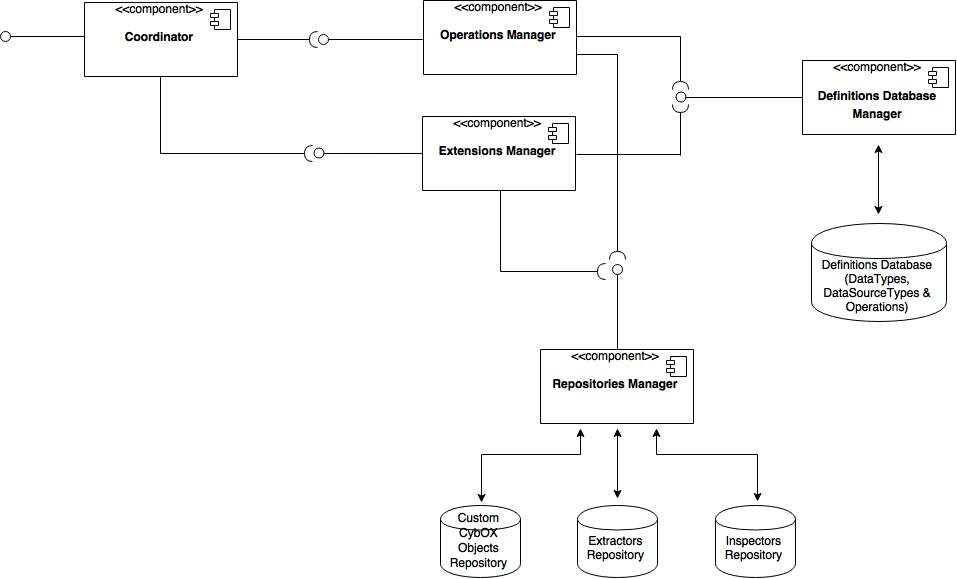
\includegraphics[scale=0.40]{figures/diagrama_de_componentes}
        \caption{Diagrama de componentes del sistema}
        \label{DiagramaComponentes}
    \end{center}
\end{figure}

A continuación veremos en detalle cada uno de los componentes del sistema.

\subsubsection{Coordinator}
Se encarga de brindar en forma de fachada todos los comandos disponibles de la herramienta, los cuales permiten llevar a cabo los casos de uso vistos. Además, es el responsable de desplegar información al usuario en la ejecución de los mismos.
\newline

\begin{python}[title=Interfaz Coordinator, captionpos=b]
set_device_info(device_info: DeviceInfo)
list_operations(data_type: string, data_source: DataSource,
                device_info: DeviceInfo)
execute_operations(names: list(string), device_info: DeviceInfo)
add_ext(type: string, def_path: string)
rm_ext(type:string, name: string)
\end{python}

\textbf{Descripción de los métodos} \newline
Los métodos brindados corresponden a los comandos del sistema ya descritos en la sección de Casos de Uso.

\subsubsection{OperationsManager}
Se encarga de responder a consultas realizadas por el usuario sobre operaciones del sistema [Req. A2] y también de crear las instancias de las operaciones que son solicitadas por el Coordinator. Luego, el Coordinator se encarga de ejecutar dichas instancias de manera batch almacenando de forma organizada los resultados de cada operación [Req. A3].
\newline

\begin{python}[title=Interfaz OperationsManager, captionpos=b]
get_operations_info(data_type: string, data_source: DataSource, 
                    device_info: DeviceInfo): list(OperationInfo)
get_operation(name: string): Operation
\end{python}

\textbf{Descripción de los métodos} \newline
El método \texttt{get\_operations\_info} obtiene la información de las operaciones que cumplen con los valores recibidos.

El método \texttt{get\_operation} se encarga de crear una instancia de la operación correspondiente al nombre indicado y la devuelve.

\subsubsection{DefinitionsDatabaseManager}
Se encarga de facilitar la interacción con la base de datos de definiciones, de manera que ayuda a los componentes OperationsManager y ExtensionsManager a cumplir con los requerimientos [Req. A2], [Req. A3] y [Req. B].
\newline

\begin{python}[title=Interfaz DefinitionsDatabaseManager, captionpos=b]
query_operations_info(data_type: string, data_source: DataSource, 
                      device_info: DeviceInfo): list(OperationInfo)
get_operation_info_by_id(id: integer): OperationInfo
get_data_type_custom_cybox_object_name(dt_name: string): string
get_data_source_type_extractor_name(dst_name: string): string
get_operation_inspector_name(op_name: string): string 
get_operation_exec_info(name: string): string,string, dict(string)
exists_operation(name: string): bool
exists_data_type(data_type: string): bool
exists_data_source_type(data_source_type: string): bool
has_all_required_param_values(data_source: DataSource): bool
add_operation(name: string, data_type_id: integer,
              data_source_type_id: integer,
              inspector_id: string,
              param_values: dict(string), 
              device_models: list(string),
              android_versions: list((string, string))
              ): bool
remove_operation(name: string): bool
add_data_type(name: string, cybox_object_name: string): bool
remove_data_type(name: string): bool
add_data_source_type(name: string,
                     extractor_name: string,
                     required_params: dict(string)
                     ): bool
remove_data_type(name: string): bool
\end{python}

\textbf{Descripción de los métodos} \newline
Los métodos \texttt{query\_operations\_info} y \texttt{get\_operation\_info\_by\_id} se encargan de realizar una consulta a la base de datos de definiciones para obtener la información de las operaciones que cumplen con los parámetros recibidos.

Los métodos \texttt{get\-\_data\-\_type\-\_custom\-\_cybox\-\_object\-\_name}, \texttt{get\-\_data\-\_source\-\_type\-\_extractor\-\_name} y \texttt{get\-\_operation\-\_inspector\-\_name} se encargan de obtener el nombre del módulo Python que implementa la extensión correspondiente.

El método \texttt{get\-\_operation\-\_exec\-\_info} se encarga de obtener los datos necesarios para ejecutar la operación cuyo nombre coincida con el recibido por parámetro.

Los métodos \texttt{exists\_operation}, \texttt{exists\_data\_type} y \texttt{exists\-\_data\-\_source\-\_type} se encargan de consultar por la existencia de operaciones, tipos de datos y tipos de fuentes de datos respectivamente.

El método \texttt{has\_all\_required\_param\_values} se encarga de verificar que una fuente de datos cuenta con valores para todos los parámetros requeridos por el tipo de dicha fuente de datos.

Los métodos con prefijo \texttt{add} se encargan de agregar definiciones de operaciones, tipos de datos y tipos de fuentes de datos a la base de datos definiciones, mientras que los métodos con prefijo \texttt{remove} se encargan de eliminar las mismas de la base de datos.

\subsubsection{ExtensionsManager}
Se encarga de gestionar los puntos de extensibilidad del sistema de forma de satisfacer el requerimiento [Req. B].
\newline

\begin{python}[title=Interfaz ExtensionsManager, captionpos=b]
add_ext(type: string, def_path: string)
rm_ext(type: string, name: string)
\end{python}

\textbf{Descripción de los métodos} \newline
El método \texttt{add\_ext} se encarga de validar la definición de la extensión recibida y añadirla al sistema, mientras que el método \texttt{rm\_ext} es responsable de eliminar la extensión indicada.

\subsubsection{RepositoriesManager}
Se encarga de gestionar el almacenamiento de los archivos que contienen las clases utilizadas por las diversas extensiones del sistema. Para esto, maneja un repositorio para cada tipo de extensión. Además, tiene la responsabilidad de cargar en tiempo de ejecución clases a partir de sus archivos correspondientes almacenados en los repositorios y devolver instancias de las mismas.
\newline

\begin{python}[title=Interfaz RepositoriesManager, captionpos=b]
add_file(repo_name: string, file_path: string)
remove_file(repo_name: string, file_name: string)
get_extractor_instance(name: string): Extractor
get_inspector_instance(name: string): Inspector
\end{python}

\textbf{Descripción de los métodos} \newline
El método \texttt{add\_file} recibe el nombre de un repositorio y la ruta al archivo a agregar, y se encarga de copiar dicho archivo al repositorio indicado.

El método \texttt{remove\_file} recibe el nombre de un repositorio y el nombre del archivo a remover, y se encarga de buscar y eliminar del repositorio correspondiente al archivo indicado.

Los métodos \texttt{get\_extractor\_instance} y \texttt{get\_inspector\_instance} devuelven una instancia de la clase correspondiente.

\section{Almacenamiento de datos}
\subsection{Repositorios} \label{repositorios}
La herramienta cuenta con varios repositorios, o en otras palabras directorios, en donde se almacenan artefactos de las extensiones del sistema (aquellas definidas en Req. B). Concretamente se cuenta con tres repositorios:

\begin{enumerate}
\item \textbf{Custom CybOX objects}: Utilizado para almacenar las clases que implementan custom cybox objects para representar nuevos tipos de datos.
\item \textbf{Extractors}: Utilizado para almacenar las clases que implementan los extractors para cada tipo de fuente de dato.
\item \textbf{Inspectors}: Utilizado para almacenar las clases que implementan los inspectors para cada operación.
\end{enumerate}

\subsection{Base de datos}
Utilizaremos una base de datos para persistir las definiciones que describen los diversos tipos de datos, tipos de fuentes de datos y operaciones disponibles en el sistema (estos son los tres puntos en los cuales podemos extender el sistema). A dicha base de dato le llamaremos \emph{DefinitionsDB}.

A continuación veremos en detalle la información almacenada para cada uno de los distintos puntos de extensión.
\newline

\begin{figure}[H]
    \begin{center}
        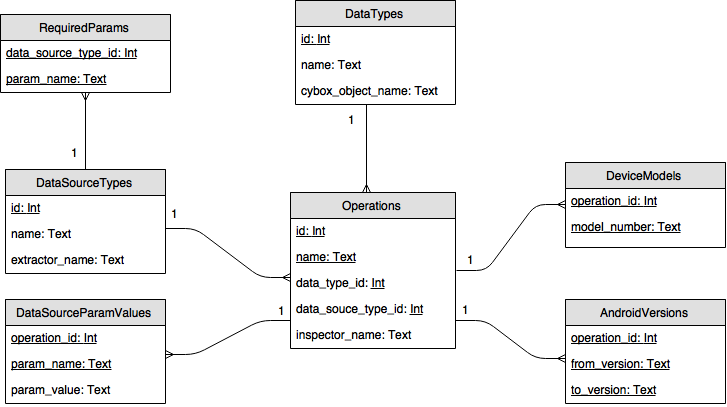
\includegraphics[width=\textwidth]{figures/esquema_de_base_de_datos}
        \caption{Esquema de la base de datos de definiciones}
    \end{center}
\end{figure}

A continuación describimos cada una de las tablas que vemos en el modelo.

\subsubsection{Tabla Operations}

\footnotesize
    \renewcommand*{\arraystretch}{1.4}
    \begin{longtable}{ | >{\bfseries}m{4cm} | >{\itshape}m{1.0cm} | >{\itshape}m{6.0cm} | >{\itshape}c |}
    \hline
    \BlackCell{Columna} & \BlackCell{Tipo de dato} & \BlackCell{Descripción} \\ \hline \hline
    id & Integer & Identificador de la operación. \\ \hline
    name & Text & Nombre de la operación. \\ \hline
    data\_type\_id & Integer & Identificador del tipo de dato de la operación. \\ \hline
    data\_source\_type\_id & Integer & Identificador del tipo de la fuente de datos de la cual la operación extrae los datos. \\ \hline
    inspector\_name & Text & Nombre del inspector utilizado por la operación para examinar los datos extraídos. \\ \hline
    \caption {Tabla Operations}
    \end{longtable}
    \normalsize
    
Esta tabla almacena el conjunto de operaciones del sistema. Es utilizada al momento de realizar la consulta que determina cuales son las operaciones que corresponden con el pedido del usuario. El identificador \emph{id} de esta tabla es usado a nivel de la base de datos para identificar a la operación. Por otro lado, el campo \emph{name} también identifica a la operación, pero es usado a nivel de usuario para consultar y ejecutar las mismas.

\subsubsection{Tabla DataTypes}
\footnotesize
    \renewcommand*{\arraystretch}{1.4}
    \begin{longtable}{ | >{\bfseries}m{3.7cm} | >{\itshape}m{1.0cm} | >{\itshape}m{6.0cm} | >{\itshape}c |}
    \hline
    \BlackCell{Columna} & \BlackCell{Tipo de dato} & \BlackCell{Descripción} \\ \hline \hline
    id & Integer & Identificador del tipo de datos. \\ \hline
    name & Text & Nombre del tipo de datos. \\ \hline
    cybox\_object\_name & Text & Nombre del objeto CybOX que representa el tipo de datos. \\ \hline
    \caption {Tabla DataTypes}
    \end{longtable}
    \normalsize
    
Esta tabla almacena los tipos de datos soportados por el sistema.

\subsubsection{Tabla DataSourceTypes}
\footnotesize
    \renewcommand*{\arraystretch}{1.4}
    \begin{longtable}{ | >{\bfseries}m{3cm} | >{\itshape}m{1.0cm} | >{\itshape}m{6.0cm} | >{\itshape}c |}
    \hline
    \BlackCell{Columna} & \BlackCell{Tipo de dato} & \BlackCell{Descripción} \\ \hline \hline
    id & Integer & Identificador del tipo de fuente de datos. \\ \hline
    name & Text & Nombre del tipo de fuente de datos. \\ \hline
    extractor\_name & Text & Nombre del extractor que implementa el mecanismo de extracción de datos para este tipo de fuente de datos. \\ \hline
    \caption {Tabla DataSourceTypes}
    \end{longtable}
    \normalsize

Esta tabla almacena los tipos de fuentes soportados por el sistema. Junto al nombre de la fuente de datos, se guarda el nombre del script que realiza la extracción de dicha fuente. Este último nombre será utilizado para realizar la búsqueda del script en el momento de ejecutar una operación.

\subsubsection{Tabla RequiredParams}
\footnotesize
    \renewcommand*{\arraystretch}{1.4}
    \begin{longtable}{ | >{\bfseries}m{4cm} | >{\itshape}m{1.0cm} | >{\itshape}m{6.0cm} | >{\itshape}c |}
    \hline
    \BlackCell{Columna} & \BlackCell{Tipo de dato} & \BlackCell{Descripción} \\ \hline \hline
    data\_source\_type\_id & Integer & Identificador del tipo de fuente de datos. \\ \hline
    param\_name & Text & Nombre del parámetro requerido por este tipo de fuente de datos. \\ \hline
    \caption {Tabla RequiredParams}
    \end{longtable}
    \normalsize
    
Esta tabla almacena los parámetros requeridos de las fuentes de datos del sistema. Al agregar una nueva operación la cual utilice una fuente de datos existente, se valida que la nueva operación especifique valores para todos los parámetros de la fuente de datos.

\subsubsection{Tabla DataSourceParamValues}
\footnotesize
    \renewcommand*{\arraystretch}{1.4}
    \begin{longtable}{ | >{\bfseries}m{2.3cm} | >{\itshape}m{1.0cm} | >{\itshape}m{6.0cm} | >{\itshape}c |}
    \hline
    \BlackCell{Columna} & \BlackCell{Tipo de dato} & \BlackCell{Descripción} \\ \hline \hline
    operation\_id & Integer & Identificador de la operación a la cual están asociados estos valores de parámetros. \\ \hline
    param\_name & Text & Nombre del parámetro. \\ \hline
    param\_value & Text & Valor del parámetro. \\ \hline
    \caption {Tabla DataSourceParamValues}
    \end{longtable}
    \normalsize
    
Esta tabla almacena los valores de parámetros requeridos por el tipo de fuente de datos asociado a la operación indicada. Para ello, se indica para cada nombre de parámetro su correspondiente valor.

\subsubsection{Tabla AndroidVersions}
\footnotesize
    \renewcommand*{\arraystretch}{1.4}
    \begin{longtable}{ | >{\bfseries}m{2.3cm} | >{\itshape}m{1.0cm} | >{\itshape}m{6.0cm} | >{\itshape}c |}
    \hline
    \BlackCell{Columna} & \BlackCell{Tipo de dato} & \BlackCell{Descripción} \\ \hline \hline
    operation\_id & Integer & Identificador de la operación a la cual está asociado este rango de versiones de Android soportadas. \\ \hline
    from\_version & Text & Versión inicial del rango. \\ \hline
    to\_version & Text & Versión final del rango. \\ \hline
    \caption {Tabla AndroidVersions}
    \end{longtable}
    \normalsize
    
Esta tabla se utiliza para almacenar las versiones de Android soportadas por las operaciones. Cuando se agrega una nueva operación, se insertan nuevos registros en esta tabla con los rangos de las versiones de Android indicados.

\subsubsection{Tabla DeviceModels}
\footnotesize
    \renewcommand*{\arraystretch}{1.4}
    \begin{longtable}{ | >{\bfseries}m{2.8cm} | >{\itshape}m{1.0cm} | >{\itshape}m{6.0cm} | >{\itshape}c |}
    \hline
    \BlackCell{Columna} & \BlackCell{Tipo de dato} & \BlackCell{Descripción} \\ \hline \hline
    operation\_id & Integer & Identificador de la operación a la cual está asociado este modelo de dispositivo soportado. \\ \hline
    model\_number & Text & Número del modelo del dispositivo soportado. \\ \hline
    \caption {Tabla DeviceModels}
    \end{longtable}
    \normalsize

Esta tabla se utiliza para almacenar los distintos dispositivos soportados por las operaciones. Cuando se agrega una nueva operación, se insertan nuevos registros en esta tabla con los modelos de dispositivos indicados.

\section{Descripción de los comandos}
\subsection*{SetDeviceInfo}
El comando permite indicarle al sistema la información del dispositivo que va a ser utilizado. Esto resulta muy útil al trabajar en el modo interactivo ya que evita que tengamos que indicar esta información como parámetro a los comandos \texttt{list} y \texttt{execute} cada vez que los deseamos utilizar. En caso que se le indique de todas formas como parámetro la información del dispositivo a estas operaciones y ya hayamos utilizado el comando \texttt{set\_device\_info}, la información indicada por parámetro será la considerada por el comando.

\subsection*{List}
El comando es de utilidad al trabajar en modo interactivo para consultar las operaciones disponibles en el sistema y obtener información de las mismas antes de utilizarlas \hyperref[reqA2]{(Req. A2)}.

Los parámetros de este comando (\emph{data\_type}, \emph{source\_type}, \emph{source\_params}, \emph{model} y \emph{version}) actúan como filtros de búsqueda. Esto es, si a un parámetro se le indica un valor, se retornarán sólo aquellas operaciones que lo cumplen. En caso de dejar vacío un parámetro, no estamos imponiendo condición alguna sobre el mismo.

\subsection*{Execute}
El comando es utilizado con el objetivo de ejecutar un conjunto de operaciones \hyperref[reqA3]{(Req. A3)}, tanto en modo interactivo como en modo batch. De esta forma, el comando recibe la lista de los nombres de las operaciones a ejecutar y la información del dispositivo. En caso de estar ejecutando en modo interactivo, la especificación de la información del dispositivo es opcional si el comando \texttt{set\_device\_info} fue ejecutado previamente.

Para cada operación se indica si la misma tuvo éxito o no. En caso de éxito, se indica el directorio en que fueron almacenados los datos resultantes de la operación, mientras que en caso de falla se indica el motivo de la misma.

\subsection*{AddExt \& RmExt}
El comando \texttt{add\_ext} nos permite agregar extensiones al sistema, mientras que el comando \texttt{rm\_ext} nos permite removerlas. Ambos reciben como parámetro el tipo de extensión (operación, tipo de dato o tipo de fuente de datos). En el caso de adición de una nueva extensión, el comando recibe una ruta al archivo de definición del mismo. En el caso de supresión de una extensión, el comando recibe el nombre de la extensión que deseamos remover.
\newline

Por más detalles sobre el funcionamiento de los comandos recién descritos, en el apéndice \ref{diagramasFlujo} se encuentran los diagramas de flujo de cada comando.

\section{Extensibilidad de la herramienta}
\label{extensibilidadDeLaHerramienta}
Uno de los requerimientos fundamentales planteados [Req. B] es que la herramienta sea fácilmente extensible. Lo que buscamos con esto es permitir que la incorporación de nuevas operaciones se pueda realizar de forma habitual, de manera que sea posible contar con un conjunto de operaciones actualizado para enfrentar las necesidades del momento.

Para lograr esto, analizamos las etapas en que consiste una operación y buscamos modelar la misma de forma de facilitar la reutilización de partes que puedan ser compartidas. Esto permite reducir el esfuerzo requerido para desarrollar una nueva operación.

Dada la naturaleza del proceso que implica una operación (como vimos en la sección Conceptos Fundamentales), podemos distinguir las siguientes etapas:
\begin{enumerate}
\item Extracción de los datos.
\item Examinación de los datos extraídos.
\item Presentación de la información encontrada.
\end{enumerate}

En la primera etapa, la operación extrae datos de una determinada fuente. Podemos notar que aquellas operaciones que obtienen datos de fuentes del mismo tipo (e.g. Aplicaciones), utilizan el mismo mecanismo (a menos de unos parámetros) para realizar la extracción. Este mecanismo es a lo que llamamos \textbf{extractor}.

En la segunda etapa, la operación examina los datos extraídos (en la etapa anterior) en busca de información de un cierto tipo de datos. Podemos notar que para este procedimiento es necesario que la operación conozca tanto la fuente de datos de donde provienen los datos extraídos como el tipo de dato que debe buscar. Esto lo hace una parte característica de la operación, y en consecuencia, no tiene sentido que sea reutilizado por otras operaciones. Al mismo le llamamos \textbf{inspector}.

En la tercera etapa, la operación organiza toda la información obtenida de forma de presentársela al usuario. Para esto, la información encontrada sobre los datos examinados es representada utilizando objetos CybOX y almacenada en archivos XML, mientras que los datos extraídos son almacenados en su forma original.

Ahora, vistas las distintas etapas que involucra una operación, vemos que podemos modelar la misma de forma que conste de dos componentes fundamentales antes mencionados: un extractor y un inspector. Contar con esta separación nos brinda lo siguiente:

\begin{itemize}
\item En primer lugar, permite que operaciones que utilicen el mismo tipo de fuente de datos hagan uso de un mismo extractor. De esta forma, al desarrollar operaciones podemos reutilizar este componente.
\item En segundo lugar, permite que el desarrollador de la operación no deba encargarse de organizar la información obtenida (tanto datos obtenidos por el extractor como datos examinados por el inspector), siendo la herramienta quien almacena de forma uniforme estos datos para todas las operaciones.
\end{itemize}

Con esto, acabamos de ver el punto de extensión más importante que brinda la herramienta, es decir, la posibilidad de extender el conjunto de operaciones con que cuenta la herramienta. Además, la herramienta también brinda otros dos puntos de extensión que permiten que podamos ampliar la diversidad de operaciones. Estos son:
\begin{itemize}
\item El conjunto de tipos de fuentes de datos. Este punto de extensibilidad permite que podamos definir operaciones que obtengan datos de nuevas fuentes de datos.
\item El conjunto de tipo de datos. Este punto de extensibilidad permite que podamos definir operaciones que buscan, examinan y representan nuevos tipos de datos.
\end{itemize}

A continuación veremos en más detalle cada uno de estos tres puntos de extensión que brinda la herramienta.

\subsection{Tipo de dato}
La información obtenida por una operación sobre un tipo de dato es representada utilizando un objeto CybOX. Como hemos visto, el lenguaje CybOX cuenta con un conjunto de objetos predefinidos capaces de representar información sobre ciertos tipos de datos.

Si deseamos desarrollar una operación que examina un tipo de dato que CybOX es capaz de representar por defecto, la herramienta también lo soporta (al utilizar el módulo CybOX que nos provee esta funcionalidad). De esta forma, la base de datos es inicializada con las definiciones de los tipos de datos correspondientes a los objetos predefinidos en CybOX.

Sin embargo, si deseamos desarrollar una operación que examina un tipo de dato que CybOX no soporta por defecto, será necesario crear un nuevo tipo de dato para representar esta información.

\subsection{Tipo de fuente de datos}
Como vimos, las fuentes de datos de un mismo tipo utilizan un mismo mecanismo de extracción de datos. El extractor es el responsable de implementar dicho mecanismo de extracción.

\subsection{Operación}
Una operación, además de extraer los datos, examina los mismos. Para eso, tiene asociado un inspector, que es quién implementa la examinación de los datos para el tipo de dato de la operación.
